\documentclass[12pt,a4paper]{article}
\usepackage[utf8]{inputenc}
\usepackage[T1]{fontenc}
\usepackage{lmodern}
\usepackage{amsmath,amssymb}
\usepackage{siunitx}
\usepackage{geometry}
\usepackage{hyperref}
\usepackage{enumitem}
\usepackage{tikz}
\geometry{margin=2.2cm}

\title{Lecture 5 -- Comparators, Schmitt Triggers, Integrators, Multivibrators}
\author{Readable Assignment Set}
\date{}

\begin{document}
\maketitle
\tableofcontents

\section{Assignments}
\subsection{E1}
Why is frequency compensation omitted in comparator integrated circuits?

\subsection{E2}
Find threshold voltages and sketch transfer characteristic for Schmitt-trigger circuits in Fig. P12.8. Comparator output levels are \(+\SI{10}{V}\) and \(-\SI{10}{V}\).

\subsection{E3}
Integrator followed by comparator with $V_{SAT}^+=\SI{14}{V}$, $V_{SAT}^- = \SI{-13}{V}$, and ideal A1/A2 unless noted. Given: 
$C=\SI{47}{nF}$, $R_1=\SI{30}{k\Omega}$, $R_2=\SI{10}{k\Omega}$, $R_3=\SI{47}{k\Omega}$, $R_4=\SI{270}{k\Omega}$.
\begin{enumerate}
\item Find comparator thresholds (symbolic and numeric), sketch $e_{o2}(e_{o1})$ and hysteresis $V_H$.
\item Sketch $e_{o1}(t)$ and $e_{o2}(t)$ over at least two periods.
\item Find frequency of $e_{o1}$.
\item Include diode forward drop $V_D=\SI{0.7}{V}$ and find percentage frequency error relative to (3).
\end{enumerate}

\subsection{E4}
Astable multivibrator with asymmetric output required: \SI{1}{kHz} and pulse/pause ratio 4:1. Pulse means $V_{SAT}^+$ and pause means $V_{SAT}^-$. Given ideal A1 except $V_{SAT}^+=-V_{SAT}^-=\SI{10}{V}$, $R_3=\SI{20}{k\Omega}$, $R_4=\SI{5}{k\Omega}$, $C=\SI{0.01}{\micro F}$, ideal diodes. Find $R_1$, $R_2$, and sketch $e_o$, $e_-$, $e_+$.

\subsection{E5}
Triangle/square-wave generator (A1, A2): $V_{SAT}^+=-V_{SAT}^-$. For ideal op-amps in (1)--(2):
\begin{enumerate}
\item Sketch $e_1$ and $e_2$ together and indicate slopes and levels symbolically.
\item Find square-wave frequency symbolically.
\item Show symbolically how frequency is affected by $V_{OS}$, $I_{OS}$, and $I_B$ for A1.
\end{enumerate}

\section{Hints}
\begin{itemize}
\item Comparator ICs prioritize speed; compensation reduces bandwidth and slew response.
\item In Schmitt triggers, thresholds are set by positive feedback divider and output saturation levels.
\item Integrator slope is $\mathrm{d}v/\mathrm{d}t=-v_{in}/(RC)$.
\item Oscillation period is total charge time between upper/lower comparator thresholds.
\item Non-ideal diode drops and op-amp offsets shift thresholds and effective charging currents.
\end{itemize}

\section{Step-by-step solutions}
\subsection{E1}
Compensating capacitors intentionally slow the device to ensure stable linear closed-loop amplification. Comparators are normally used open-loop in switching mode where maximum speed is desired, so internal frequency compensation is usually omitted to keep propagation delay and transition time low.

\subsection{E2}
\begin{enumerate}
\item For each Schmitt topology, write threshold node equation using $V_{SAT}^+=+10\,\text{V}$ and $V_{SAT}^-=-10\,\text{V}$.
\item Compute upper threshold $V_{TH+}$ when output is high and lower threshold $V_{TH-}$ when output is low.
\item Hysteresis width is $V_H=V_{TH+}-V_{TH-}$.
\item Draw transfer characteristic with two switching points and output saturating at $\pm\SI{10}{V}$.
\end{enumerate}

\subsection{E3}
\begin{enumerate}
\item Comparator thresholds:
\[
V_{TH\pm}=\pm \beta V_{SAT}\quad\text{(with possible asymmetry due to }+14\text{ and }-13\text{ V levels)}.
\]
Use resistor divider around A2 to compute exact $\beta$ and separate positive/negative thresholds.
\item Integrator slope with comparator output level $V_{drive}$:
\[
\frac{\mathrm{d}e_{o1}}{\mathrm{d}t}=-\frac{V_{drive}}{R_{in}C}.
\]
Use piecewise slopes for positive and negative drive levels.
\item Half-period is threshold excursion divided by slope magnitude; period is sum of both halves. Frequency is $f=1/T$.
\item With diode drop $V_D$, effective charging/discharging voltages change to $(V_{drive}-V_D)$ or $(V_{drive}+V_D)$ depending on direction; recompute $T$ and 
\[
\%\,\text{error}=\frac{|f_{ideal}-f_{VD}|}{f_{ideal}}\cdot100\%.
\]
\end{enumerate}

\subsection{E4}
\begin{enumerate}
\item Enforce duty relation $t_{pulse}:t_{pause}=4:1$ and total period $T=\SI{1}{ms}$.
\item Thus $t_{pulse}=\SI{0.8}{ms}$ and $t_{pause}=\SI{0.2}{ms}$.
\item For each interval, write capacitor charging/discharging equation through the active resistor path (set by diode orientation and selected resistor).
\item Solve two timing equations for $R_1$ and $R_2$.
\item Sketch waveforms showing comparator output square wave and capacitor ramp between threshold levels.
\end{enumerate}

\subsection{E5}
\begin{enumerate}
\item Comparator output $e_2$ toggles between $\pm V_{SAT}$; integrator output $e_1$ is triangular between Schmitt thresholds.
\item Slopes are $\pm V_{SAT}/(RC)$ scaled by input network factors.
\item With symmetric thresholds $\pm V_T$, half-period is $t_h=2V_T/(V_{SAT}/RC)=2V_TRC/V_{SAT}$, so 
\[
f=\frac{1}{2t_h}=\frac{V_{SAT}}{4V_TRC}.
\]
\item Include non-ideal A1 by replacing effective threshold and integrator drive with shifted values from $V_{OS}$ and bias-current-induced node voltages; then linearize to obtain sensitivity terms $\partial f/\partial V_{OS}$, $\partial f/\partial I_B$, $\partial f/\partial I_{OS}$.
\end{enumerate}

\subsection{Conceptual timing sketch}
\begin{center}
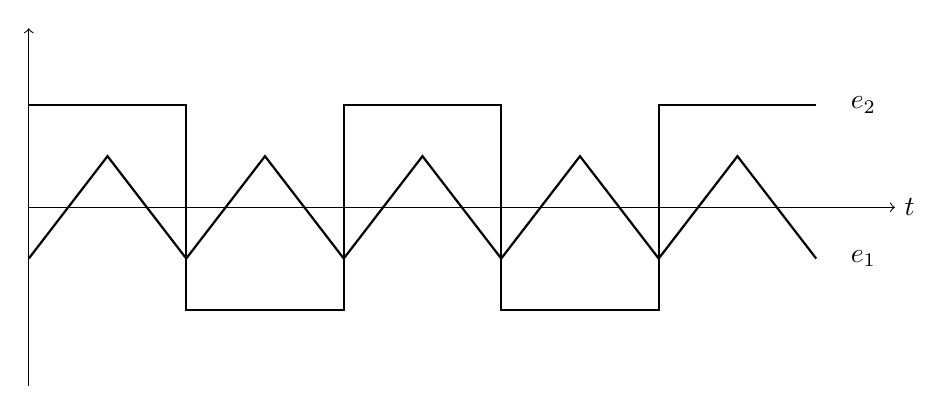
\begin{tikzpicture}[xscale=1.0,yscale=0.65]
\draw[->] (0,0) -- (11,0) node[right] {$t$};
\draw[->] (0,-3.5) -- (0,3.5);
\draw[thick] (0,2) -- (2,2) -- (2,-2) -- (4,-2) -- (4,2) -- (6,2) -- (6,-2) -- (8,-2) -- (8,2) -- (10,2);
\node at (10.6,2) {$e_2$};
\draw[thick] (0,-1) -- (1,1) -- (2,-1) -- (3,1) -- (4,-1) -- (5,1) -- (6,-1) -- (7,1) -- (8,-1) -- (9,1) -- (10,-1);
\node at (10.6,-1) {$e_1$};
\end{tikzpicture}
\end{center}

\end{document}
